\section{Physikalische Grundlagen}
\subsection{Der piezoelektrische Effekt}
Das Wort \textit{\glqq piezo\grqq{}} stammt vom griechischen Wort \textit{\glqq pi\'{e}zein = drücken\grqq{}} ab. Erstmals wurde der piezoelektrische Effekt 1880 durch die Brüder Pierre und Jacques Curie entdeckt.\autocites[vgl.][]{duden01}[vgl.][]{Curie}\\
Wird ein Kristallgitter durch äußeren Druck verformt, entsteht an den Oberflächen eine elektrische Ladung \textit{Q}. Dies führt zu einer messbaren Spannung. Die erzeugte Ladung \textit{Q} ist direkt proportional  zum Druck \textit{p}, der einwirkenden Fläche \textit{A} sowie dem stoffabhängigen Piezomodul \textit{k}:
\begin{eqnarray}
    Q=k \cdot A \cdot p
\end{eqnarray}
In Abbildung \ref{fig:piezoeffekt} ist der Piezoeffekt am Kristallgitter von $SiO_2$ dargestellt. Abhängig von der Druckachse zur polaren Achse des Kristalls unterscheidet man zwischen dem longitudinalen (\ref{fig:piezoeffekt}b) oder dem transversalen Effekt (\ref{fig:piezoeffekt}c). Vorallem letzterer findet in der Praxis Anwendung. Piezoelektrische Sensoren weisen aufgrund ihrer geringen Temperaturabhängigkeit hohe Messgenauigkeiten auf. Hauptsächlich werden diese Sensoren in dynamischen Messungen mit hohen Messfrequenzen eingesetzt. \autocites[vgl.][260 \psqq]{Sensoren}[vgl.][273 \psq]{Physik}

\begin{figure}[H]
   \centering
    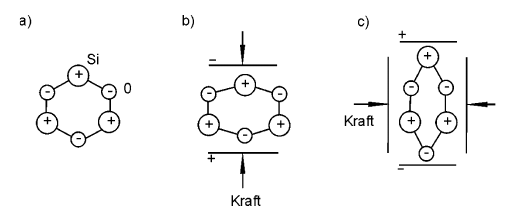
\includegraphics[scale=0.6]{Bilder/Piezoeffekt.png}
    \caption[Darstellung des Piezoeffekts]{Piezoeffekt am Kristallgitter von $SiO_2$ \footnotemark}
    \label{fig:piezoeffekt}
\end{figure}
\footnotetext{\cite{Physik}}
Die Umkehrung des piezoelektrischen Effekts, auch \textit{Elektrostriktion} genannt, ist ebenso möglich. Hier wird eine elektrische Feldstärke \textit{E} an einen geeigneten Kristall angelegt. Dies führt zu einer Längenänderung \textit{$\epsilon$}. \autocite[vgl.][274]{Physik} Die bekannteste Anwendung dieses Effekts ist der Injektor zum Einspritzen von Dieselkraftstoffen. Hierbei sind mehrere Piezoelemente in Reihe als sogenannte Stacks geschalten und bewirken bei Anlegung einer Spannung den Nadelhub der Einspritzdüse. Der piezoelektrische Effekt lässt sich somit als Sensor und Aktor nutzbar machen. 
%------------------------------------------------------------------------------
%------------------------------------------------------------------------------
%------------------------------------------------------------------------------
\subsection{Grundlagen der Strömungsmechanik}
In der Strömungsmechanik, vor allem in Rohrleitungen, unterscheidet man zwischen laminaren (geschichteten) und turbulenten (ungeordneten) Strömungen. Bei einer laminaren Strömung fließen die Fluidteilchen in Hauptstromrichtung ohne Querbewegungen. In turbulenten Strömungen werden die Fluidteilchen aufgrund von Reibungskräften zusätzlich quer zur Hauptströmung abgelenkt. Dadurch entstehen Wirbel. Für die Beschreibung der Strömung wurde die dimensionslose Reynolds-Zahl \textit{Re} eingeführt. Sie beschreibt das Verhältnis der kinetischen Energie und der Reibungsenergie:
\begin{eqnarray} \label{for:Re}
    Re &=&\frac{\rho \cdot L \cdot u}{\eta}\\
    mit: \quad \rho &=& Dichte \nonumber \\
    L &=& L\ddot{a}nge~ des ~umstr\ddot{o}mten ~ K\ddot{o}rpers \nonumber \\
    u &=& Str\ddot{o}mungsgeschwindigkeit \nonumber \\
    \eta &=& Z\ddot{a}higkeit ~ des ~ Mediums  \nonumber
\end{eqnarray}
In Rohrleitungen liegt für kleine Reynolds-Zahlen von $Re = 100$ bis $Re_{krit} = 2320$ eine laminare Strömung vor. Für $Re > 2320 $ treten mit steigender $Re$ immer stärkere Wirbel auf und die Strömung wird turbulent. Für umströmte Profilkörper variiert die kritische Reynolds-Zahl $Re_{krit}$. \autocites[vgl.][63]{Physik}[vgl.][342]{Böge} \\
Wird ein Körper umströmt, so entstehen an seinen Ablösepunkten Wirbelablösungen. Ab einer Reynolds-Zahl von $Re \approx 40$ bis $Re = 2 \cdot 10^5$ treten die Wirbel periodisch auf. Dieses Phänomen wird nach seinem Entdecker Theodor von K\'{a}rm\'{a}n (1881-1963) auch als K\'{a}rm\'{a}n`sche Wirbelstraße bezeichnet (siehe Abbildung \ref{fig:wirbelstrasse}, Seite \pageref{fig:wirbelstrasse}). \autocite[vgl.][441 \psq]{Surek}

\begin{figure}[H]
   \centering
    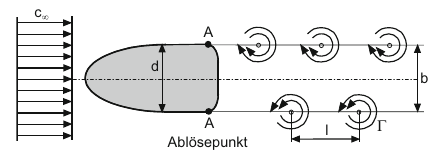
\includegraphics[scale=0.75]{Bilder/Wirbelstrasse.png}
    \caption[K\'{a}rm\'{a}n`sche Wirbelstraße]{K\'{a}rm\'{a}n`sche Wirbelstraße an einem umströmten Körper \footnotemark}
    \label{fig:wirbelstrasse}
\end{figure}
\footnotetext{\cite[][442]{Surek}}
Eine weitere dimensionslose Zahl ist die Strouhal-Zahl. Sie ist als Verhältnis der lokalen zur konvektiven Beschleunigung definiert:\autocite[vgl.][352]{Böge}
\begin{eqnarray}\label{for:Sr}
    Sr&=&\frac{f \cdot d}{u}\\
    mit: \quad f &=& Abl\ddot{o}sefrequnez \land d = K\ddot{o}rperdicke \land \nonumber \\
    u &=& Str\ddot{o}mungsgeschwindigkeit \nonumber
\end{eqnarray}
In Abbildung \ref{fig:re_sr} ist die Abhängigkeit der Strouhal-Zahl $Sr$ von der Reynolds-Zahl $Re$ dargestellt. Im Bereich von $Re \approx 100$ bis $Re \approx 2 \cdot 10^5$ ist die Strouhal-Zahl $Sr \approx 0,2$. Dieser Umstand wird sich bei Wirbelstromzählern zunutze gemacht. Mithilfe der gemessenen Ablösefrequenz $f$ und der bekannten Staukörperdicke lässt sich die Anströmgeschwindigkeit $u$ ermitteln. \autocite[vgl.][442]{Surek}

\begin{figure}[H]
    \centering
    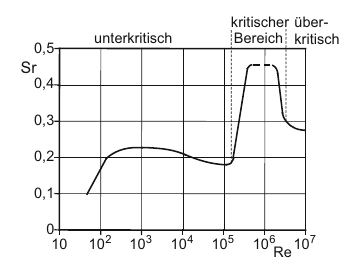
\includegraphics[scale=0.75]{Bilder/Re_Sr.png}
    \caption[Strouhal-Zahl in Abhängigkeit der Reynolds-Zahl]{Strouhal-Zahl Sr in Abhängigkeit der Reynolds-Zahl Re\footnotemark}
    \label{fig:re_sr}
\end{figure}
\footnotetext{\cite[][442]{Surek}}
%Mit den bisher vorgestellten physikalischen Grundlagen der Strömungsmechanik lässt sich im Folgenden die Funktionsweise eines Wirbelstromzählers beschreiben.
%------------------------------------------------------------------------------
%------------------------------------------------------------------------------
%------------------------------------------------------------------------------



